\documentclass[]{article}





%Need to turn back into a two-column confrence paper for submission
%\documentclass[]{ieeetran}






\usepackage[margin=1in]{geometry}
\usepackage{physics}
\usepackage{amsmath, amsfonts, amssymb}
\usepackage{nccmath}
\usepackage{cuted}
\usepackage{mathtools}
\usepackage{hyperref}
\usepackage{empheq}
\usepackage{graphicx}

% MATLAB Formating Code
\usepackage[numbered,framed]{matlab-prettifier}
\lstset{style=Matlab-editor,columns=fullflexible}
\renewcommand{\lstlistingname}{Script}
\newcommand{\scriptname}{\lstlistingname}



%opening
\title{MECH 6327 Project Report:\\
Examining Discrete-Time Polytopic Linear Parameter-Varying Systems under threat of malicious actuator and sensor manipulation}
\author{Jonas Wagner}
\date{2021 May 14}

\begin{document}

\maketitle

\begin{abstract}
	In this project they dynamics of Discrete-Time Polytopic Linear Parameter-Varying (LPV) Systems will be examined. Specifically, various methods for the dual state and parameter estimation will be reproduced with the intent of analyzing effectiveness of these observers against various attacks. Each method performs optimization to minimize the estimation error in various ways while remaining stable and achieving certain performance criteria. Potentially the reachability of the system may be determined for various fault and attack scenarios through the minimization of an ellipsoidal bound.
\end{abstract}


\newpage
\tableofcontents


\newpage
\section{Polytopic Systems Background}
Polytopic LPV system models are essentially a smooth interpolation of a set of LTI submodels constructed using a specified weighting function. This can be looked at as decomposing a system into multiple operating spaces that operate as linear submodels. It is possibile for a Polytopic model to take a complex nonlinear model and redefine it as a time-varying interpolation of multiple linear submodels.

Section references:\footnote{Each subsection is mostly a summary of sections from these sources but with elaboration and consistent notation.}
\cite{beelen2017joint} \cite{ORJUELA2019295} \cite{orjuela2013nonlinear}\\

\subsection{General Continuous Time Polytopic Model} 
The simple polyotopic LPV structure can be described by the following weighted linear combination of LTI submodels:
\begin{equation}\label{eq:CT_poly_sys_def}
	\begin{cases}
		\dot{x}(t) 	= \sum_{i=1}^r \mu_i(\xi(t))\{A_i x(t) + B_i u(t)\}  \vspace{5pt} \\ 
		y(t)		= \sum_{i=1}^r \mu_i(\xi(t)) C_i x(t)
	\end{cases}
\end{equation}
with state variable $x \in \real^n$ common to all $r$ submodels, control input $u \in \real^p$, output $y \in \real^q$, weighting function $\mu_i(\cdot)$ and premise variable $\xi(t) \in \real^{w}$. 

Additionally, the weighting functions $\mu_i (\cdot)$ for each subsystem must satisfy the convex sum constraints:
\begin{equation}\label{eq:convex_sum_constraints}
	0 \leq \mu_i(\xi), \ \forall i = 1,\dots,r \ \ \text{and} \ \ \sum_{i=1} \mu_i(\xi) = 1
\end{equation}

%notes on dimensions: n = states, m = inputs, p = outputs, w = # of weights, r = # of subsystems

One notable downside, for our application, is the requirement for $\xi(t)$ to be explicitly known in real-time for the model to function. This requirement is the primary driving factor in investigating this system as when $\xi(t)$ is not explicitly known additional uncertainties now exist in a system that are open for exploitation by an attacker.


\subsection{Discrete Time Polytopic Model}
In the DT-Polytopic Model the CT-Polytopic Model, \eqref{eq:CT_poly_sys_def}, is extended into the discrete time equivalence (either through sampling and zero-order holds or by definition) by the following parameter-varying system:

\begin{equation}\label{eq:DT_poly_sys_def}
	\begin{cases}
		x_{k+1} &= \sum_{i=1}^{m} \alpha^i (A_i x_k + B_i u_k)\\
		y		&= C x_k
	\end{cases}
\end{equation}
with state variable $x \in \real^n$, control input $u \in \real^p$, and output $y \in \real^q$ common to all of the $m$ submodels. Each submodel is also associated with state matricies $A_i$ and $B_i$ while the output is calculated from the actual state by matrix $C$.

The scheduling parameter, $\alpha \in \mathcal{A}$ is unknown and time-varying, with $\mathbf{A}$ defined as:
\begin{equation}\label{eq:alpha_set}
	\mathcal{A} = \{\alpha\in \real^m \ | \ \sum_{i=1}^m \alpha^i = 1, \ \alpha^i \geq 0 \ \ \forall \ i \in \{1,2,\dots,m\}\}
\end{equation}
%notes on dimensions: n = states, m = inputs, p = outputs, N = # of subsystems

In the discrete time case, the unknown scheduling parameter, $\alpha$, is problematic for when developing a state-estimator, thus a Joint State-Parameter estimator must be used. The discrete nature of the measurements may also prove to be even more problematic if an attack is injected in any discrete measurement.

\newpage
\section{Joint State-Parameter Estimation Problem}
The problem of developing joint state and parameter estimator is defined as finding recursive update rules to ensure that state and parameter estimates approach the actual states and parameters. This can be described as finding $f_x$ and $f_\alpha$ such that
\begin{equation}\label{eq:est_pblm_statement}
	\begin{cases}
		\hat{x}_{k+1} 		&= f_x(\hat{x}_k, \hat{\alpha}_k, \{u_l, y_l\}_{l=\bar{k}_x})\\
		\hat{\alpha}_{k+1} 	&= f_\alpha(\hat{x}_k, \hat{\alpha}_k, \{u_l, y_l\}_{l=\bar{k}_\alpha})
	\end{cases}
\end{equation}
with $\bar{k}_x, \bar{k}_\alpha < k$ result in $\norm{x_k - \hat{x}_k} \to 0$ and $\norm{\alpha - \hat{\alpha}_k} \to 0$ as $k \to \infty$.

\subsection{Problem Simplifications/Assumptions \cite{beelen2017joint}}
For simplicity, and probably for feasibility reasons, the following assumptions will also be made:

\begin{enumerate}
	\item $\alpha \in \mathcal{A}$ is constant (or at least slowly time-varying)
	\item The estimated system is observable $\forall \ \hat{\alpha} \in \mathcal{A}$, (i.e. $(\sum_{i=1}^m \hat{\alpha} A_i, C)$ is an observable pair)
	\item A unique solution exists to the joint-estimation problem
\end{enumerate}
$C \qty(q I - \sum_{i=1}^{m} \alpha^i A_i x_k)^{-1} \sum_{i=1}^m \alpha^i B_i \\= C \qty(q I - \sum_{i=1}^{m} \hat{\alpha}^i A_i x_k)^{-1} \sum_{i=1}^m \hat{\alpha}^i B_i \implies \alpha = \hat{\alpha}$

\subsection{Potential Methods}
Three joint state and parameter estimator methods for LPV systems will be developed and tested for the ability of each to react to malicious input and measurement interference.
The three estimation methods of interest 
%\footnote{taken directly from \cite{beelen2017joint} and we are essentially recreating these results but performing additional tests} 
include:
\begin{enumerate}
	\item Dual-Estimation (DE) approach is a method that first solves a two step optimization problem for parameters-estimation and then uses a "traditional" robust polytopic observer design for state estimation. \cite{beelen2017joint}
	\item Extended Kalman Filter (EKF) using prediction and update steps for the system estimates, but this version does require the assumption of Gaussian noise. \cite{ekf_param_est}
	\item Interacting Multiple Model estimation (IMM) method which uses a different kalmen filter for multiple modes and the probability that the system will be a certain mode.\cite{bar2004estimation}
\end{enumerate}

\newpage
\section{Kalmen Filter Derived Methods}
\subsection{Extended Kalmen Filter (EKF) Method \cite{ekf_param_est}}
The Extended Kalmen Filter (EKF) method relies on a prediction and update steps for both state and parameter estimates by augmenting the state with the parameters creating a nonlinear system.
\begin{equation}
	\medmath{\mqty[x_{k+1}\\ \alpha_{k+1}] = \mqty[\sum_{i=1}^m \alpha^i \qty(A_i x_k + B_i u_k)\\ \alpha_k] := f(x_k, \alpha_k, u_k)}
\end{equation}
This is then solved through a two-step prediction and estimation process. The prediction step is defined as
\begin{subequations}
	\begin{align}
		\hat{x}_{k|k-1} &= \sum_{k=1}^m \hat{\alpha}_{k-1|k-1}^i \qty(A_i \hat{x}_{k-1|k-1} + B_i u_{k-1})\\
		\hat{\alpha}_{k|k-1} &= \hat{\alpha}_{k|k}\\
		P_{k|k-1} &= \hat{A}_{k-1} P_{k-1|k-1} \hat{A}_{k-1}^\intercal + Q
	\end{align}
\end{subequations}
with the update steps defined by
\begin{subequations}
	\begin{align}
		\mqty[\hat{x}_{k|k}\\ \hat{\alpha}_{k|k}] &= \mqty[\hat{x}_{k|k-1}\\ \bar{\alpha}_{k|k-1}] + L_k \qty(y_k - C \hat{x}_{k|k-1})\\
		P_{k|k} &= \qty(I - L_k \hat{C}) P_{k|k-1}
	\end{align}
	and then to restrict $\hat{\alpha}_{k|k} \in \mathcal{A}$, it is determined by
	\begin{equation}
		\hat{\alpha}_{k|k} = \arg \min_{\alpha\in\mathcal{A}} \norm{\alpha - \bar{\alpha}_{k|k}}
	\end{equation}
\end{subequations}
with the augmented estimated parameters defined by
\begin{subequations}
	\begin{align}
		L_k &= P_{k|k-1} \hat{C}^\intercal \qty(R + \hat{C} P_{k|k-1} \hat{C}^\intercal)^{-1}\\
		\hat{A}_k &= \eval{\pdv{f(x_k, \alpha_k, u_k))}{\mqty[x&\alpha]^\intercal}}_{(\hat{x}_k, \hat{\alpha}_k, u_k)}\nonumber\\
		&= \medmath{\mqty[\sum_{i=1}^m \hat{\alpha}_{k|k}^i A_i &\mqty[A_1 x_{k|k} + B_1 u_k \cdots A_m x_{k|k} + B_m u_k]
		%\qty(A_1 x_{k|k} + B_1 u_k) \cdots \qty(A_m x_{k|k} + B_m u_k)]
		\\ 0 &I]}\\
		\hat{C} &= \mqty[C &0]
	\end{align}
\end{subequations}
In this estimator, $Q$ and $R$ are Positive Semi-definite covariance matrices, traditionally corresponding to process and measurement noise estimates, and can be used as tuning parameters. However, this does require the assumption of Gaussian noise which is not always valid within the actual system.\\
This method is widely used and will converge when the state and parameter estimates are close enough and any nonlinearities are continuous, but no specific guarantees can be made about the robustness.


%\subsection{Interacting Multiple Model (IMM) Method \cite{bar2004estimation}}
%The Intercting Multiple Model (IMM) method uses a individual kalmen filters for each modes and then determines the probability that the system will be a certain mode.


\newpage
\section{DE Method Optimization Problem Definition and Solution \cite{beelen2017joint}} \label{sec:DE_method_opt_pblm}
The primary optimization problems to be analyzed are the state and parameter estimation problems within the DE method. This method separates the joint-estimation problem into a state and then a parameter-estimation problem, each of which are determined using convex optimization techniques.

The parameter estimation is done independently using a recursive parameter-estimation method relying solely on the input-output data $\{u_l , y_l\}_{l=1}^k$ without any reliance on the state-estimates. This itself is an optimization problem that aims to minimize the prediction error given the parameter estimates.

\subsection{State Estimation Problem and Solution}
The system state is estimated using a modified Luenberger observer defined by
\begin{equation} \label{eq:DE_state_observer_form}
	\hat{x}_{k+1} = \sum_{i=1}^m \hat{\alpha}_k^i \qty(A_i \hat{x}_k + B_i u_k + L_i \qty(C \hat{x}_k - y_k))
\end{equation}
with $\hat{\alpha}_k \in \mathcal{A}$ being the estimated parameters and $L_i$ being selected to ensure the estimation error, $e_k = x_k - \hat{x}_k$, is stable.

\subsubsection{State Estimation Error:}
The estimation error is defined as
\begin{equation} \label{eq:DE_state_error}
	\medmath{e_{k+1} = \sum_{i=1}^m \qty(\hat{\alpha}_k^i\qty(A_i + L_i C)e_k + \qty(\alpha^i - \hat{\alpha}_k^i)\qty(A_i x_k + B_i u_k))}
\end{equation}
A solution that ensures $e_k$ is stable is that when the disturbance caused by the deviation of $\hat{\alpha}$, $v_k$ decays to zero (a requirement for the parameter estimation problem), $e_k$ also decays to zero. This is equivelent to ensuring Input-to-State Stability (ISS) of the estimator.\\

\subsubsection{Estimator ISS Lyapanov Function:}
The estimator can be rewritten as
\begin{equation}\label{eq:DE_state_error_simple}
	e_{k+1} = \sum_{i=1}^m \hat{\alpha}_k^i \qty(A_i + L_i C) e_k + v_k
\end{equation}
and ISS with respect to the disturbance term, $v_k$, defined by
\begin{equation}
	v_k = \sum_{i=1}^m (\alpha^i - \hat{\alpha}_k^i) (A_i x_k + B_i u_k)
\end{equation}
can be guaranteed by using an ISS Lyapnov function to solve for an appropriate Luenberger gain.\\
The ISS Lyapnov function is a function $V : \real^{n+m} \to \real$, such that $$V(e,\hat{\alpha})>0 \forall e\neq 0, \quad V(0,\hat{\alpha}) = 0,$$ and

\begin{equation}
	V(e_{k+1}, \hat{\alpha}_{k+1}) - V(e_k, \hat{\alpha}_k) < -\norm{e_k}^2 + \zeta \norm{v_k}^2
\end{equation}
for all $k \in \{0, \dots,N\}$.

\newpage
\subsubsection{LMI Feasibility Problem for ISS}
%%%% Insert Derivation from the theorem taken from Heemels 2010????
A theorem provided in \cite{heemels2010} states that if there exists matrices $P_i,\ F_i,\ G_i,\ i \in \{1, \dots, m\}$ and a scaler $\zeta$ such that
\begin{equation}
	\mqty[G_i + G_i^\intercal - P_j			&0	&G_i A_i + F_i C	&G_i\\
		  0							&I	&I					&0\\
		  A_i^\intercal G_i^\intercal + C^\intercal F_i^\intercal	&I	&P_i				&0\\
		  G_i^\intercal						&0	&0					&\zeta I]
		  \succ 0
\end{equation}
for all $i, j \in \{1,\dots,m\}$, then for \eqref{eq:DE_state_error_simple} with the Luenberger gains calculated with
\begin{equation}
	L_i = G_i^{-1} F_i
\end{equation}
guarantees ISS with respect to $v$.\footnote{The derivation explained in \cite{heemels2010} is interesting (but long and more Optimal Estimation focused in nature) and essentially proves that the ISS Lyapnov function always exists if the solution is feasible.}
This essentially means that the $e_k \to 0$ whenever $v_k \to 0$, or identically, $\hat{x}_k \to x_k$ and $\hat{\alpha}_k \to \alpha_k$, over a finite number of steps.

\subsection{Parameter Estimation Problem and Solution}
The DE method estimates the parameters by using only the input-ouput data $\{u_l , y_l\}_{l=0}^k$ and completely ignores the estimated states. This is done through the minimization of the prediction error directly through an optimization based on a modified least-squares type algorithm.

\subsubsection{Parameter Estimate Optimization Problem\cite{beelen2017joint}}
The parameter-estimation problem is solved by minimizing the prediction error defined as
\begin{subequations}\label{eq:DE_param_opt_pblm_original}
	\begin{equation}
		\hat{\alpha}_k = \arg \min_{\alpha \in \mathcal{A}} \sum_{l=0}^k \gamma^{k-l} \norm{y_k - \varphi_k \nu(\alpha)}^2
	\end{equation}
	with a the forgetting factor $0<\gamma\leq1$ and
	\begin{align}
		\varphi_k &= \mqty[y_{k-1} \ \dots \ y_{k-n_x} \ u_{k-1} \ \dots \ u_{k-n_x}]\\
		\nu(\alpha) &= \mqty[a_1(\alpha) \ \dots \ a_{n_x}(\alpha) \ b_1(\alpha) \ \dots \ b_{n_x}(\alpha)]^\intercal
	\end{align}
\end{subequations}
with variables $a_i$ and $b_i$ being the coefficients from the polynomials
\begin{subequations}\label{eq:DE_param_poly}
	\begin{align}
		\sum_{i=1}^{n_x} a_i(\alpha)q^i &= \det(qI - \sum_{i=1}^m \alpha^i A_i)\\
		\sum_{i=1}^{n_x} b_i(\alpha)q^i &= C \text{adj}\qty(qI - \sum_{i=1}^m \alpha^i A_i) \sum_{i=1}^m \alpha^i B_i
	\end{align}
\end{subequations}
which are in fact the transfer function coefficients for the system itself, \eqref{eq:DT_poly_sys_def}.\\
It is also noteworthy that the optimization problem \eqref{eq:DE_param_opt_pblm_original} is a nonlinear (and possibly nonconvex) optimization problem, so instead of solving this directly, a two step approach can be taken to first solve for the coefficients in \eqref{eq:DE_param_poly} and then determining the scheduling parameter corresponding to those transfer function coefficients.

\newpage
\subsubsection{Step 1: Determine Polynomial Coefficients}
Determining the polynomial coefficients is a simple optimization problem consisting of an unconstrained linear least-squares optimization problem given by
\begin{equation}\label{eq:DE_param_opt_pblm_pt1}
	\hat{\nu}_k = \arg \min_\nu \sum_{l=0}^k \gamma^{k-l} \norm{y_k - \varphi_k \nu}^2
\end{equation}
The solution to this optimization problem can be computed recursively with
\begin{subequations}\label{eq:DE_param_opt_pblm_pt1_soln}
	\begin{align}
		P_k &= \frac{1}{\gamma} P_{k-1} - \frac{1}{\gamma} \varphi_k^\intercal \qty(\gamma I + \varphi P_{k-1} \varphi_k^\intercal)^{-1} \varphi_k P_{k-1}\\
		\hat{\nu}_k &= \hat{\nu}_{k-1} + P_k \varphi_k^\intercal \qty(y_k - \varphi_k \hat{\nu}_{k-1})
	\end{align}
\end{subequations}
with initial estimates of $\hat{\nu}_0$ and some matrix $P\succ0$.

\subsubsection{Step 2: Determine Scheduling Parameter}
The second step is to calculate parameter estimates as the solution to the nonlinear optimization problem
\begin{equation}\label{eq:DE_param_opt_pblm_pt2}
	\hat{\alpha}_k = \arg \min_{\alpha\in\mathcal{A}} \qty(\hat{\nu}_k - \nu(\alpha))^\intercal P_k^{-1} \qty(\hat{\nu}_k - \nu(\alpha))
\end{equation}
The optimal solution and resultant parameter estimates are equivalent to the optimal solution to the original optimization problem \eqref{eq:DE_param_opt_pblm_original}. The proof for this is shown in \cite{beelen2017joint} and consists of taking the solution to \eqref{eq:DE_param_opt_pblm_pt2} and going in reverse through the definition and solution of \eqref{eq:DE_param_opt_pblm_pt1} to equate the optimal solution to that of the original optimization problem \eqref{eq:DE_param_opt_pblm_original}.



\newpage
\section{Numerical Experimentation}

\subsection{Simulation Implementation}
A generalized Method in Simulink was attempted to be created that would be able to simulate an arbitrary Polytopic System, each of the estimation methods, and introduce attack vectors into the system. This is the future goal to be worked on this summer, but after spending a considerable amount of time learning how to do this, it was abandoned for the short term testing for this project and instead the "toy"/numerical DT model given in \cite{beelen2017joint} was simulated alongside each estimator in a simple MATLAB script for the entirely DT model. These MATLAB scripts can be seen in \appendixname \ \ref{apx:MATLAB}.

\subsection{Example Polyotopic System}
A simple DT Polyotopic Model taken from \cite{beelen2017joint} \ is defined by \eqref{eq:DT_poly_sys_def} with the following state-matrices:
\begin{equation}
	\begin{aligned}
		A_1 = \mqty[-0.80 & 0.25\\ 0.25 & -0.30], \ &B_1 = \mqty[1.9\\0]\\
		A_2 = \mqty[0.30 & 0.70\\ 0.70 &0], \ &B_2 = \mqty[-1\\ 1.50]\\
		A_3 = \mqty[-0.30 & 0.65\\ 0.55 &0.10], \ &B_3 = \mqty[0.30\\ -2]\\
		A_4 = \mqty[0.55 & =0.20\\ -0.40 &-0.30], \ &B_4 = \mqty[-0.60\\0]
	\end{aligned}
\end{equation}
with the output matrix $C = \mqty[0 &1]$, making the dimensions 

\subsection{DE Implementation}
%DE: \gamma = 0.9
The Dual Estimate method was implemented as explained in Section \ref{sec:DE_method_opt_pblm} was then simulated. Untimely it was very difficult to find a solver that was consistent at solving and being robust for a wider array of starting positions for the second step. Eventually it was determined that using Yalmip directly to solve the parameter problem was more effective at converging. (This primarily occurred with the first step as the update for P could result in a negative semi-definite matrix) The 'forgetting factor' from the paper was used: $$\gamma = 0.9$$

\subsection{EKF Implementation}
%EKF: R = 0.01 and Q = \mqty[0_{n\cross n} & \\ &100 * I_{m\cross m}}]
The Extended Kalmen Filter was implemented as well using the parameters from the paper:
\begin{displaymath}
	R = 0.01 \text{ and } Q = \mqty[0_{n\cross n} & \\ & 100 * I_{m \cross m}]
\end{displaymath}


%\subsection{IMM Implementation}
%%IMM: p^{ii} = 0.99 ??????????? check paper




\subsection{Recreated Results}
The results from the original paper were recreated in MATLAB (\appendixname \ref{apx:MATLAB}). The input was selected as essentially a random PWM signal of strength $u_0 = 0.5$.
Specifically, the actual system response is can be seen in \figurename \ \ref{fig:systemresponsenoattack}. Additionally, the response for the DE and EKF methods can be seen in \figurename \ \ref{fig:denoattack} \ and \figurename \ \ref{fig:ekfnoattack} \ respectively.

\begin{figure}
	\centering
	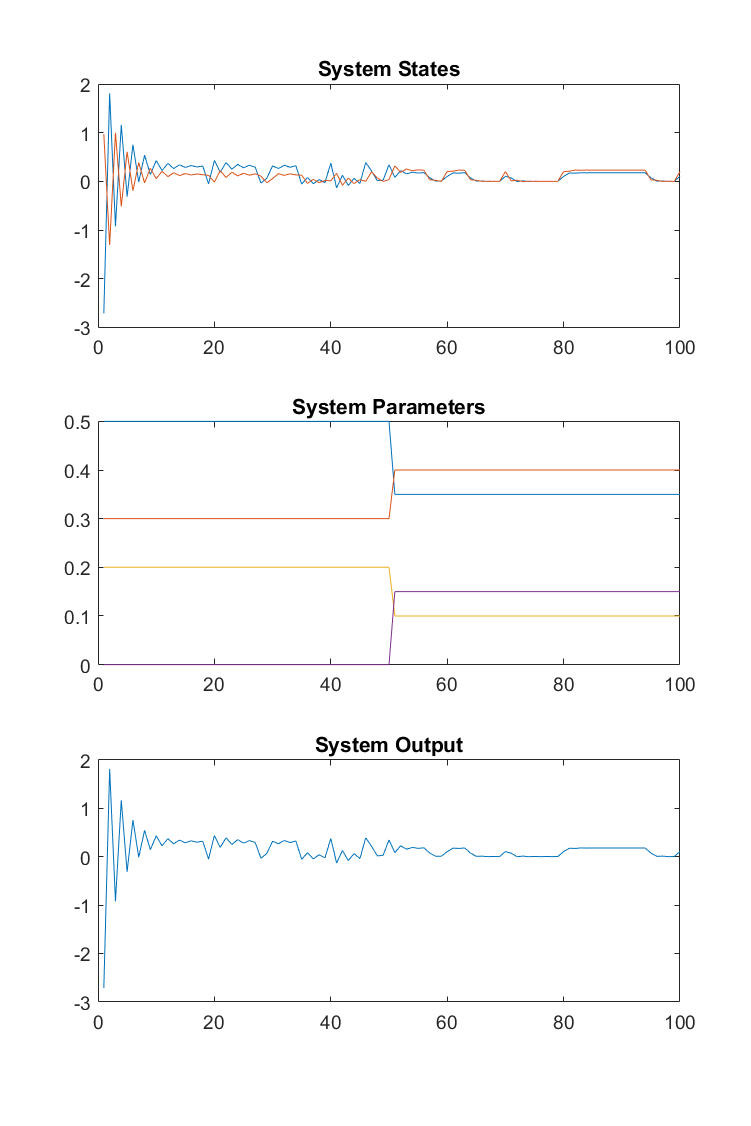
\includegraphics[width=\linewidth]{../../fig/SystemResponse_no_attack}
	\caption{Recreated System Results}
	\label{fig:systemresponsenoattack}
\end{figure}

\begin{figure}
	\centering
	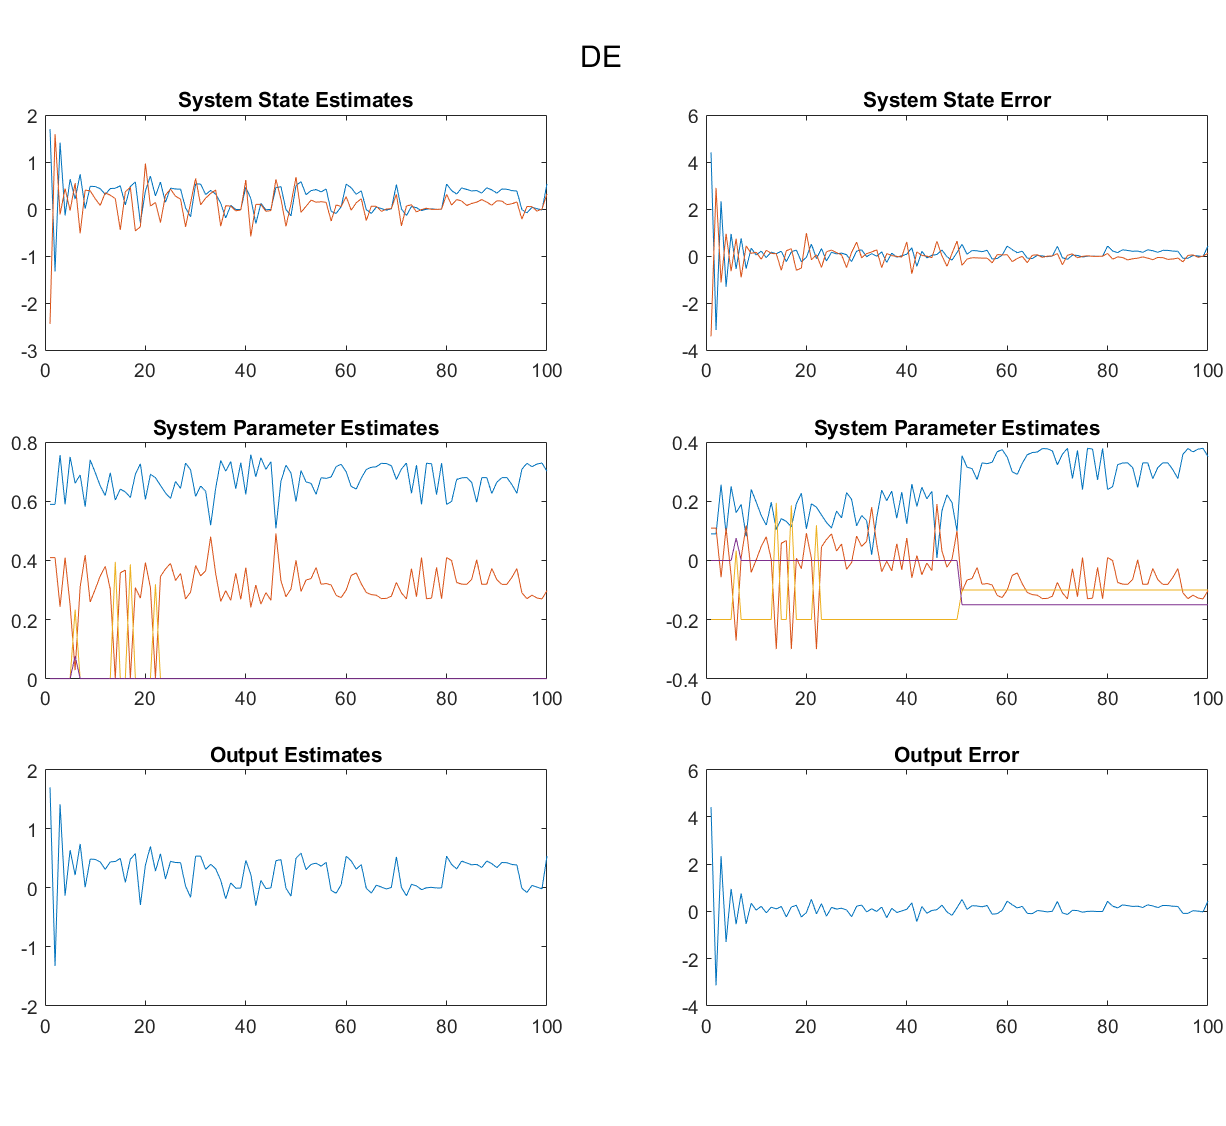
\includegraphics[width=\linewidth]{../../fig/DE_no_attack}
	\caption{Recreated DE Simulated Results}
	\label{fig:denoattack}
\end{figure}

\begin{figure}
	\centering
	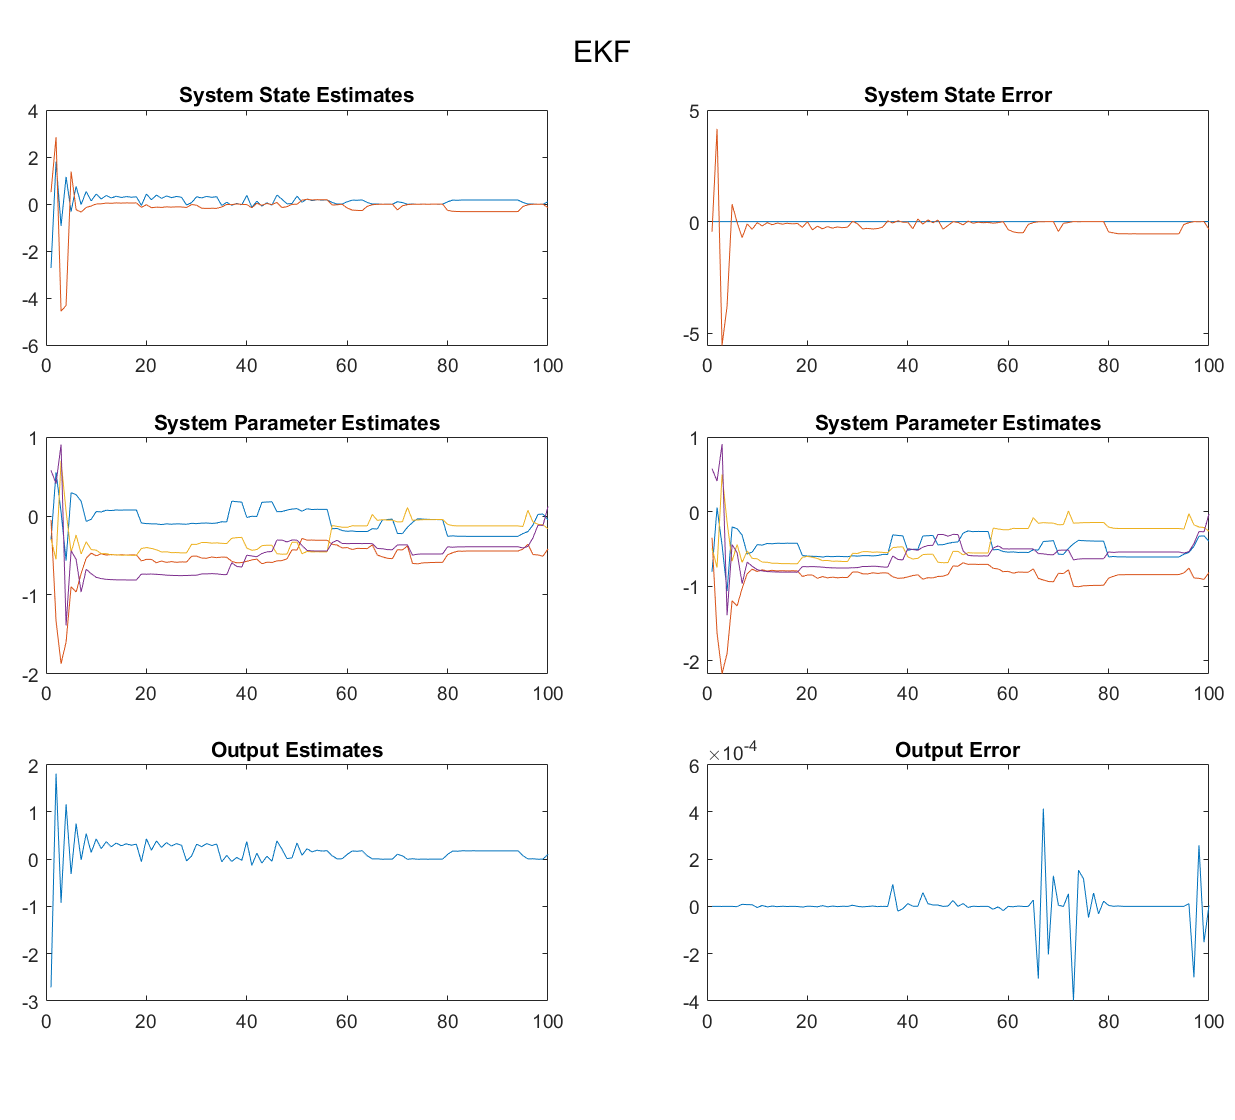
\includegraphics[width=\linewidth]{../../fig/EKF_no_attack}
	\caption{Recreated EKF Simulated Results}
	\label{fig:ekfnoattack}
\end{figure}

%\newpage
\section{Attack Implementation}
The attacks for this system were essentially Gaussian Noise. In the future a more general model (preferably in Simulink) will be developed to test this on more complicated systems, but for now a simple Gaussian noise signal was generated and applied to the measurement each time-step.

%\newpage
\section{Results and Discussion}
The results from the original paper were recreated in MATLAB (\appendixname \ref{apx:MATLAB}) and a complete collection of the plots can be seen attached in \appendixname \ref{apx:figs}. The input was selected as essentially a random PWM signal of strength $u_0 = 0.5$ and multiple power levels of gaussian (attack) noise were tested.\\
A few important examples to look at are (as expected) the noise increases, the error increases for both of the methods of estimation. One big takaway can be seen in the ability for the EKF method to work better for really small deviations, but untimely, the state estimates are not stable and the error goes to infinity, while the DE method actually guarantees feasibility and convergence.





%
%
%\newpage
%\section{Project Objectives}
%The primary objective of this project will be to reproduce three joint state and parameter estimator methods for LPV systems then test the ability of each to react to malicious input and measurement interference. A secondary/future objective will be to calculate the reachability set and how it is manipulated due to an attack on the system.
%
%The three estimation methods of interest \footnote{taken directly from \cite{beelen2017joint} and we are essentially recreating these results but performing additional tests} include:
%\begin{enumerate}
%	\item Dual-Estimation (DE) approach is a method that first solves a two step optimization problem for parameters-estimation and then uses a "traditional" robust polytopic observer design for state estimation. \cite{beelen2017joint}
%	\item Extended Kalman Filter (EKF) using prediction and update steps for the system estimates, but this version does require the assumption of Gaussian noise. \cite{beelen2017joint}
%	\item Interacting Multiple Model estimation (IMM) method which uses a different Kalmen filter for multiple modes and the probability that the system will be a certain mode.\cite{bar2004estimation}
%\end{enumerate}
% Need to find access to \cite{bar2004estimation} for the IMM algorithm details...

%The primary attack methods for initial testing (for simplicity) will consist of malicious random gaussian noise being added to measurements. The power of these attacks can be classified into three catagories depending on the malicous noise power:
%\begin{enumerate}
%	\item Stealthy attacks: power of the attack is along the same level as the normal noise standard-deviation.
%	\item Unstealthy attacks: the attack is disruptive, yet detectable, with aims to degrade the system performance.
%	\item Super Unstealthy attack: a very considerable attack that aims to severely disrupt a system while not remaining undetectable.
%\end{enumerate}
%
%The next objective will be to show how much each attack method can effect the states (specifically the reachable set) for each estimator.\footnote{and potentially develop a better solution... modifying \cite{securestateestimation}?} This work is very similar to \cite{hashemi2018comparison} but will be expanding from stochastic DT-LTI systems to deterministic DT-LPV systems.
%
%\section{Proposed Methods}
%The following steps will be taken to complete the problem.
%
%\begin{enumerate}
%	\item This project will begin by reproducing the results of joint state and parameter estimation from \cite{beelen2017joint} using the same LPV system used in the paper. (This will likely be done using Simulink with custom estimator blocks.)
%%	\item The next step will be to introduce additional system noise (presumably to the scheduling parameters themselves) and measurement poise into the sensors. This will be important to do first and perform a separate analysis of each before malicious attacks are included.
%	\item Next attacks will be introduced into the sensor and the response for each estimator will be compared.
%	\item This will then be expanded to a more interesting system\footnote{Seperator Testbed? scheduling parameters being valve on/off and for various linearized tank level systems... is it possible to analyze with a scheduling parameter dependent on a state???... Otherwise a more complicated electrical network w/ switches or pneumatic system could be done instead} that will be more useful for sensor attack testing (i.e. more sensors then states or high noise system).
%	\item Finally, an analysis of the reachable set deviation due to attacks will be performed by finding a minimal ellipsoid constraining the states that would be reachable prior to attack detection.\footnote{possibly future work}
%\end{enumerate}

%\newpage
\bibliographystyle{ieeetr}
\bibliography{mybib.bib}



\onecolumn
\newpage
\appendix
\subsection{MATLAB}\label{apx:MATLAB}
All code I wrote for this project can be found on my GitHub repository:\\
\href{https://github.com/jonaswagner2826/DT_LPV_attack_analysis}{https://github.com/jonaswagner2826/DT\_LPV\_attack\_analysis}\\
% DT_LPV_sim_script
\lstinputlisting[caption={DT\_LPV\_sim\_script}]{../../DT_LPV_sim/DT_LPV_sim_script.m}
\newpage
% DT_LPV_sim_script
\lstinputlisting[caption={alpha\_traj}]{../../DT_LPV_sim/alpha_traj.m}
\newpage
% DT_LPV_sim_script
\lstinputlisting[caption={est\_DE}]{../../DT_LPV_sim/est_DE.m}
\newpage
% DT_LPV_sim_script
\lstinputlisting[caption={est\_EKF}]{../../DT_LPV_sim/est_EKF.m}

\subsection{Complete Set of Results} \label{apx:figs}

\begin{figure}
	\centering
	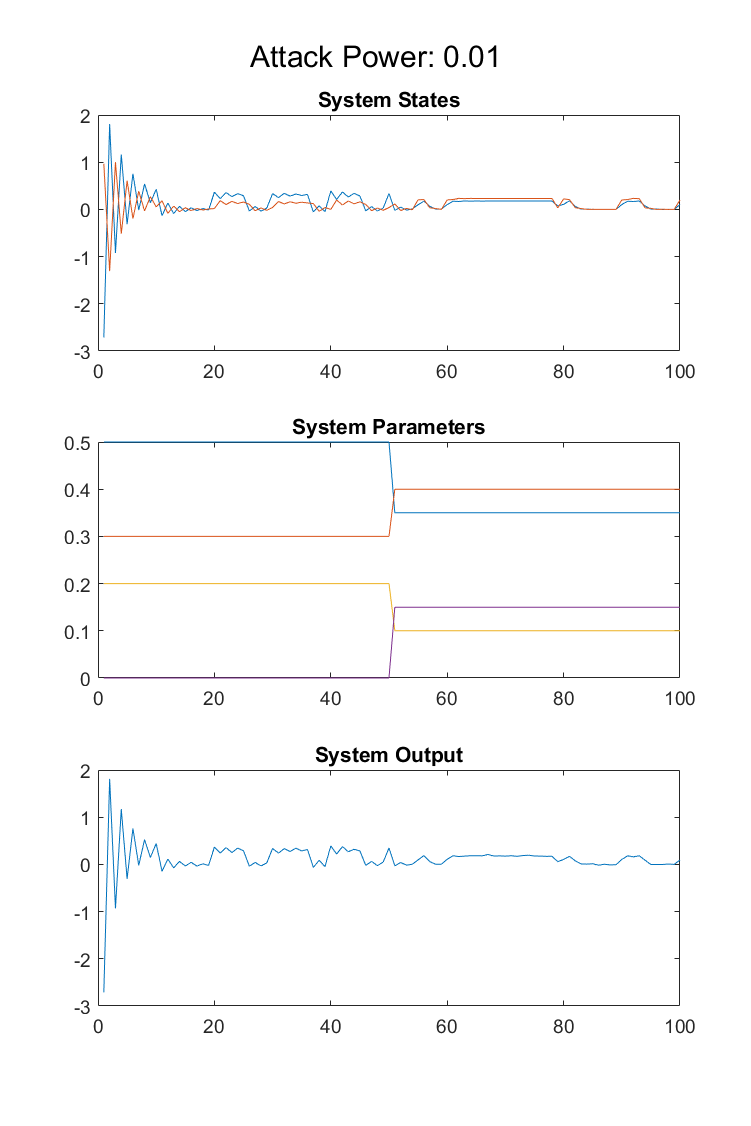
\includegraphics[width=0.7\linewidth]{../../fig/SystemResponse_attack_0_01}
	\caption{$v_0 = 0.01$ System Results}
	\label{fig:systemresponseattack001}
\end{figure}

\begin{figure}
	\centering
	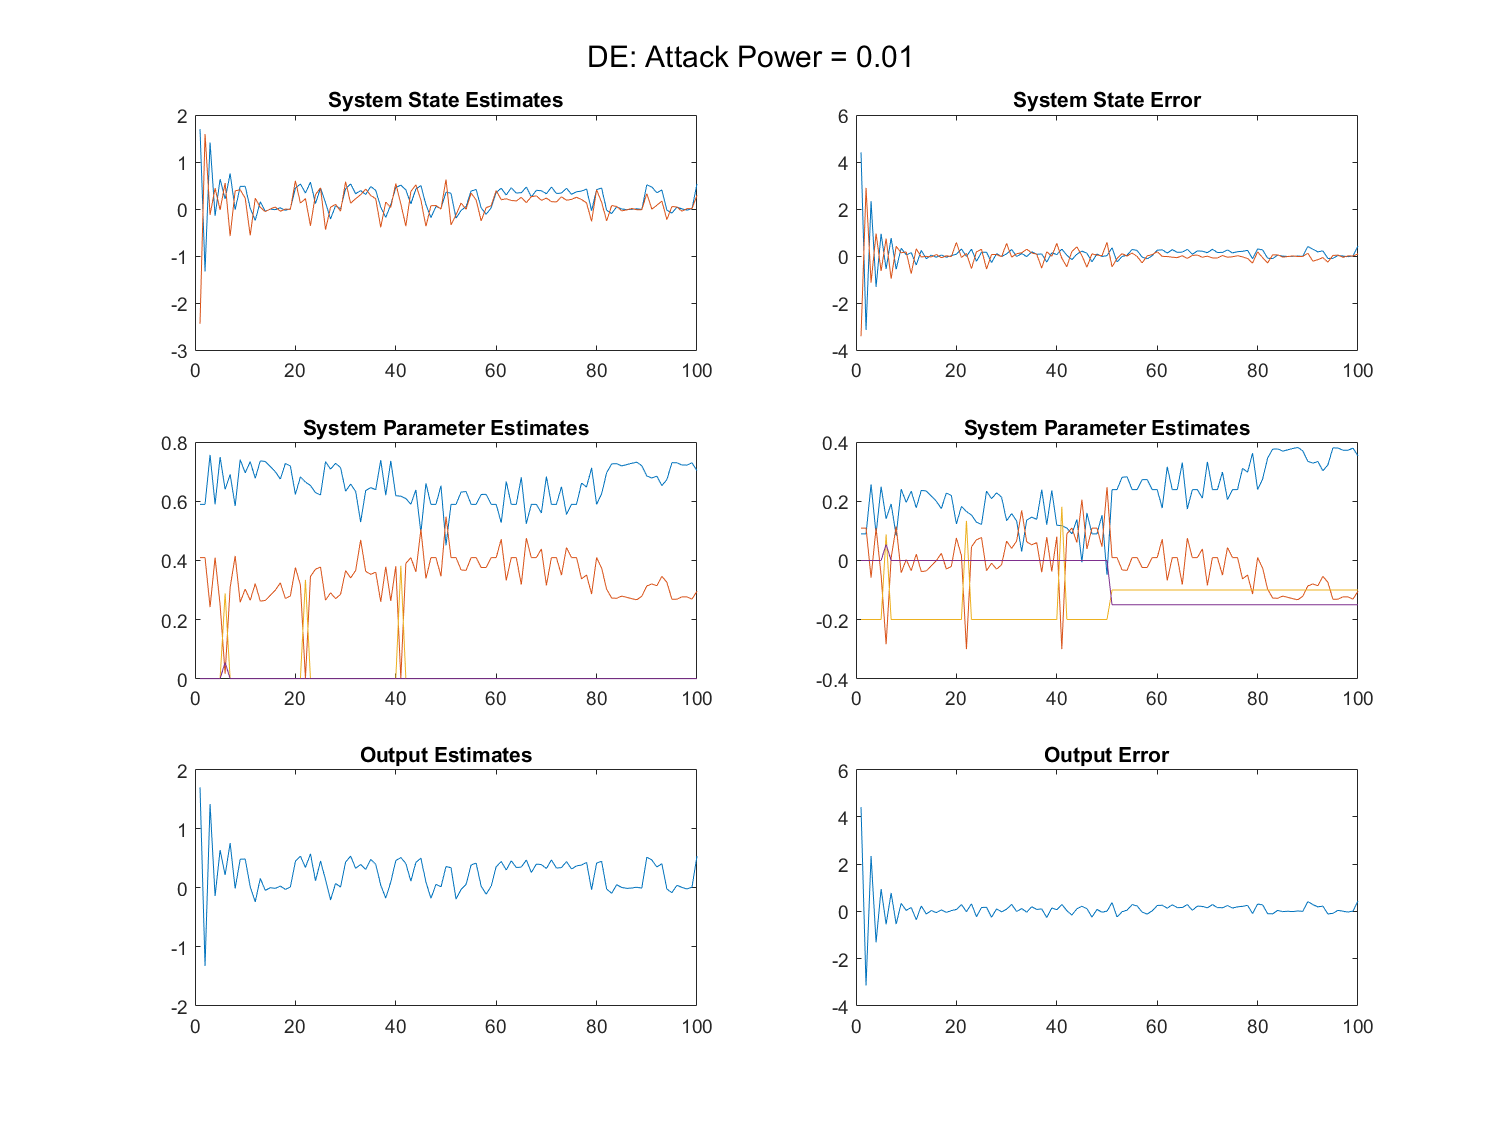
\includegraphics[width=\linewidth]{../../fig/DE_attack_0_01}
	\caption{DE with $v_0 = 0.01$ Simulated Results}
	\label{fig:deattack001}
\end{figure}

\begin{figure}
	\centering
	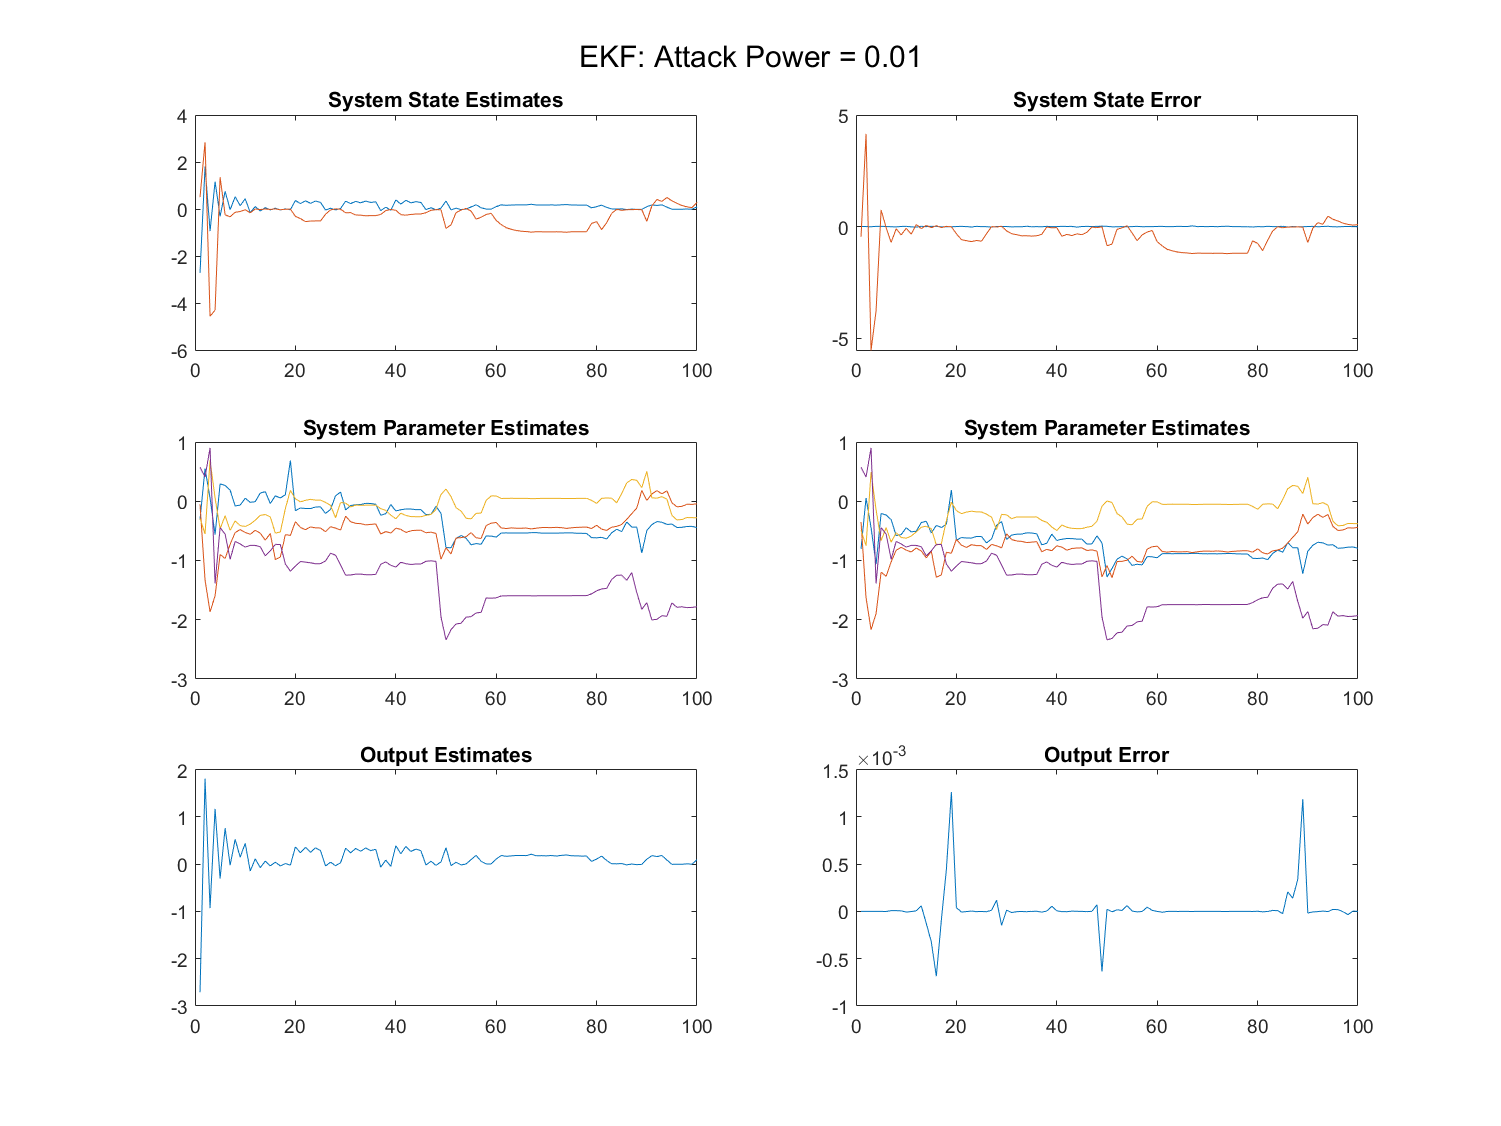
\includegraphics[width=\linewidth]{../../fig/EKF_attack_0_01}
	\caption{EKF with $v_0 = 0.01$ Simulated Results}
	\label{fig:ekfattack001}
\end{figure}

\begin{figure}
	\centering
	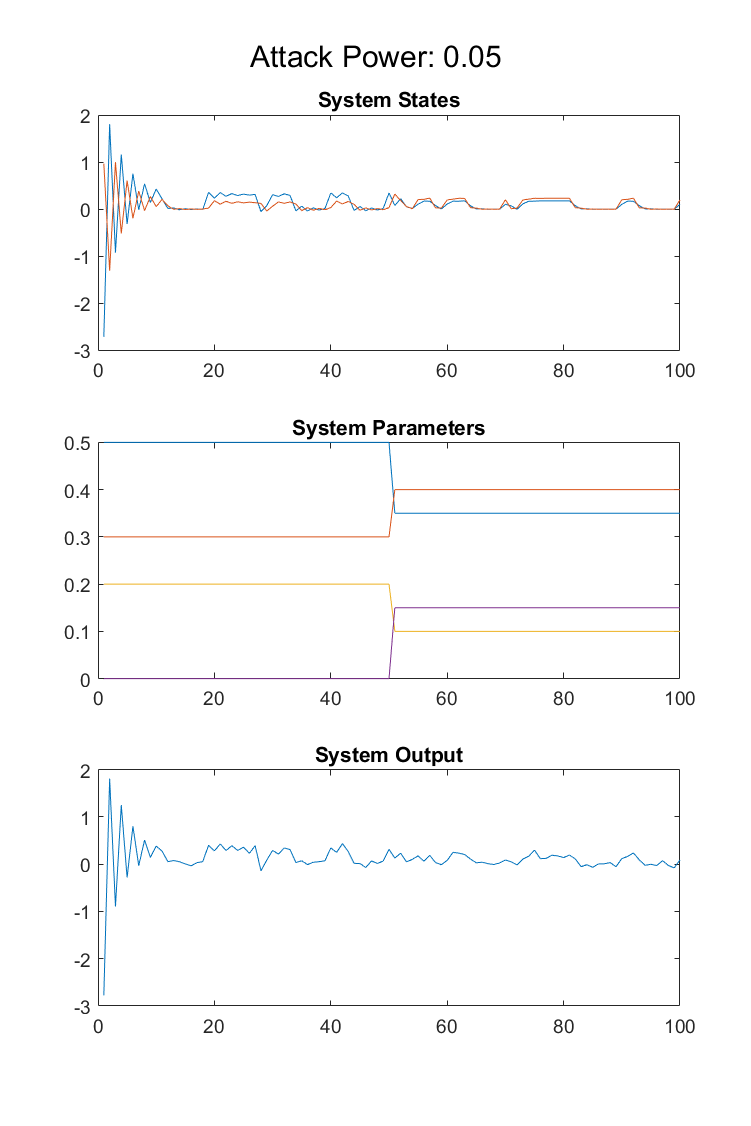
\includegraphics[width=0.7\linewidth]{../../fig/SystemResponse_attack_0_05}
	\caption{$v_0 = 0.05$ System Results}
	\label{fig:systemresponseattack005}
\end{figure}

\begin{figure}
	\centering
	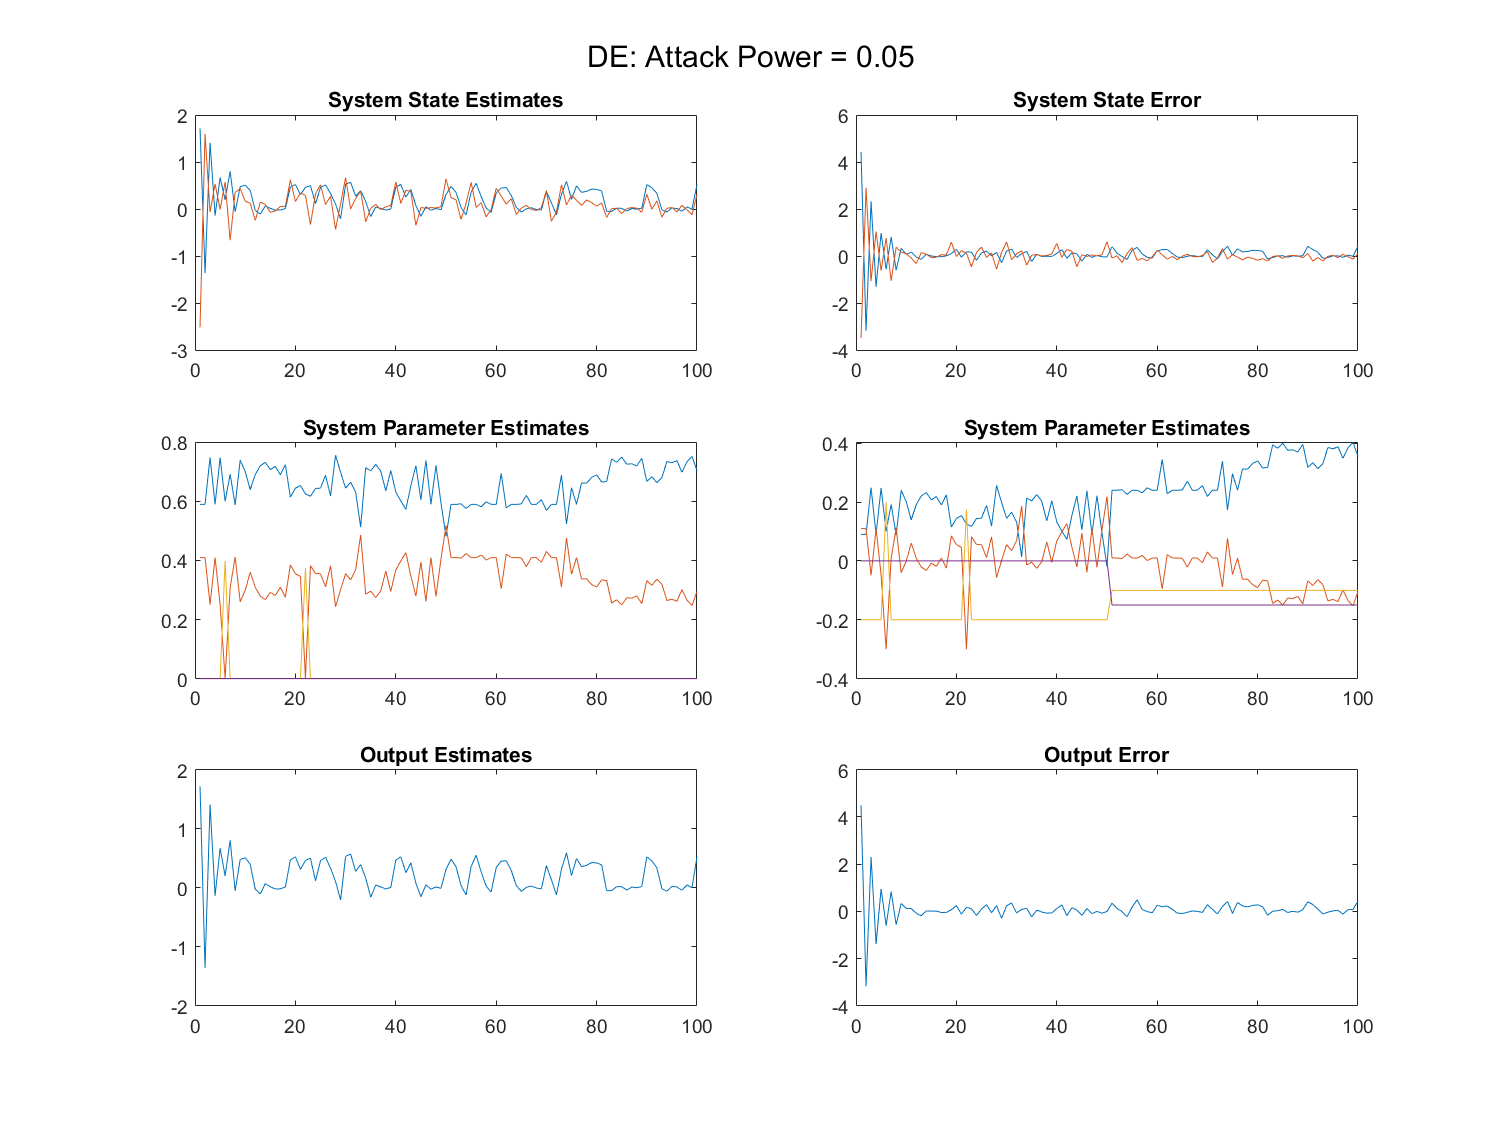
\includegraphics[width=\linewidth]{../../fig/DE_attack_0_05}
	\caption{DE with $v_0 = 0.05$ Simulated Results}
	\label{fig:deattack005}
\end{figure}

\begin{figure}
	\centering
	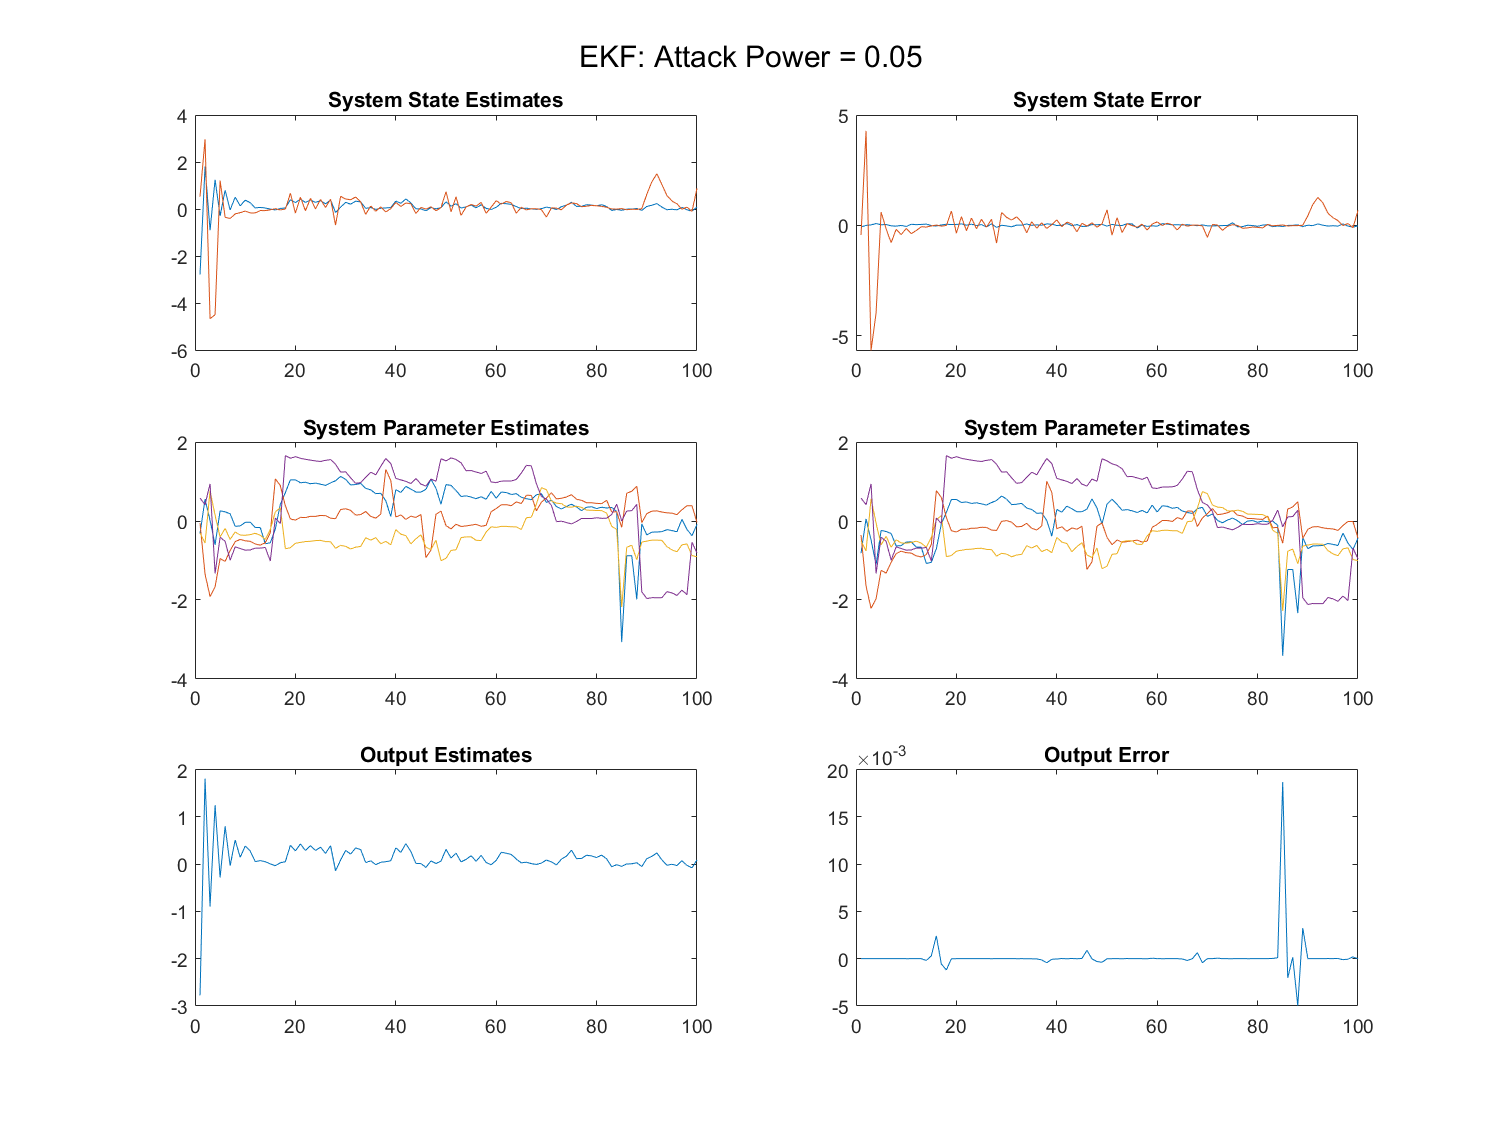
\includegraphics[width=\linewidth]{../../fig/EKF_attack_0_05}
	\caption{EKF with $v_0 = 0.05$ Simulated Results}
	\label{fig:ekfattack005}
\end{figure}

\begin{figure}
	\centering
	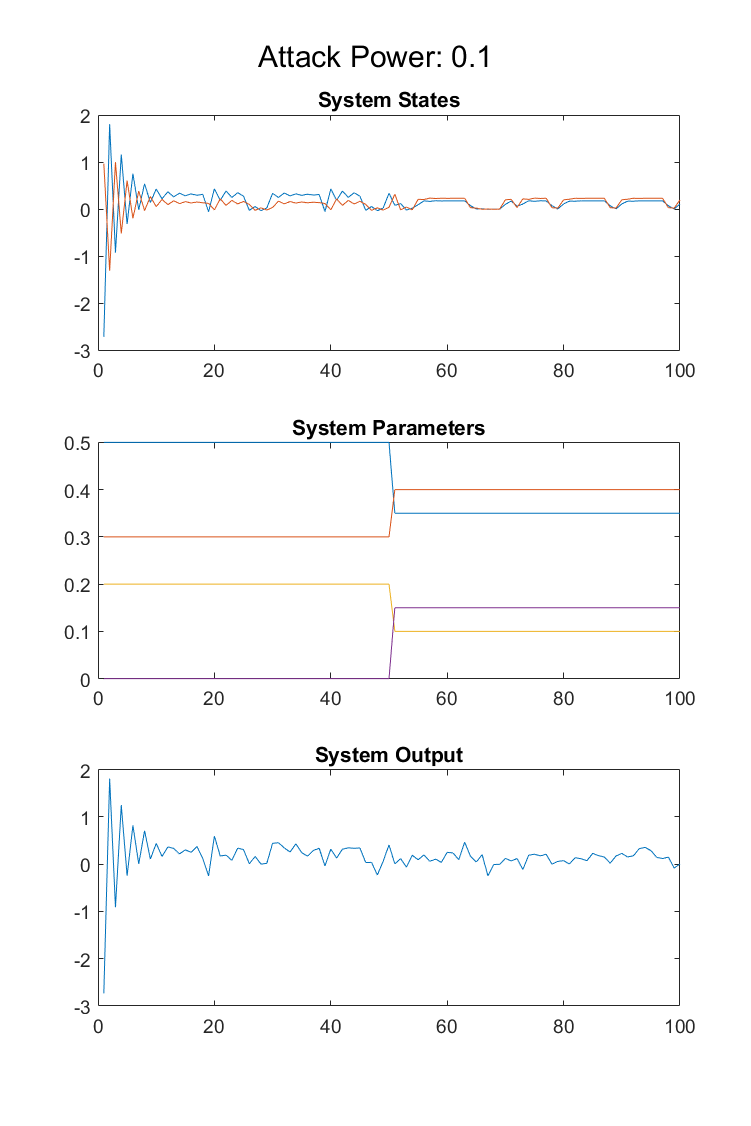
\includegraphics[width=0.7\linewidth]{../../fig/SystemResponse_attack_0_1}
	\caption{$v_0 = 0.1$ System Results}
	\label{fig:systemresponseattack01}
\end{figure}

\begin{figure}
	\centering
	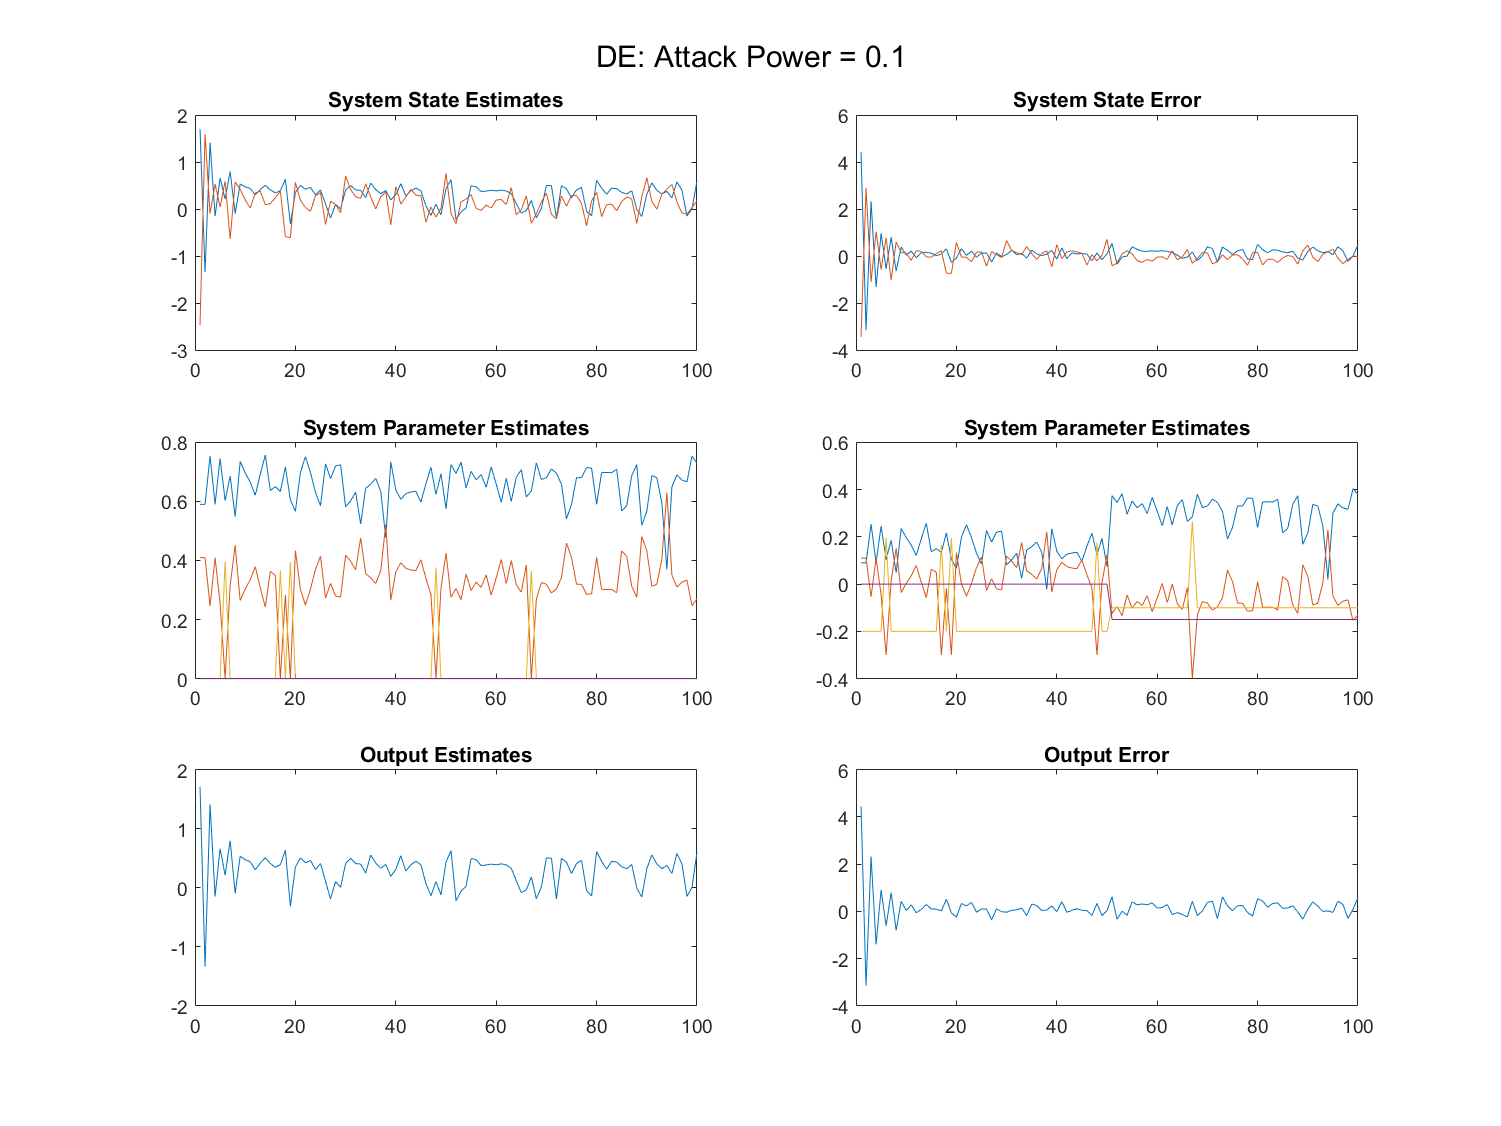
\includegraphics[width=\linewidth]{../../fig/DE_attack_0_1}
	\caption{DE with $v_0 = 0.1$ Simulated Results}
	\label{fig:deattack001}
\end{figure}

\begin{figure}
	\centering
	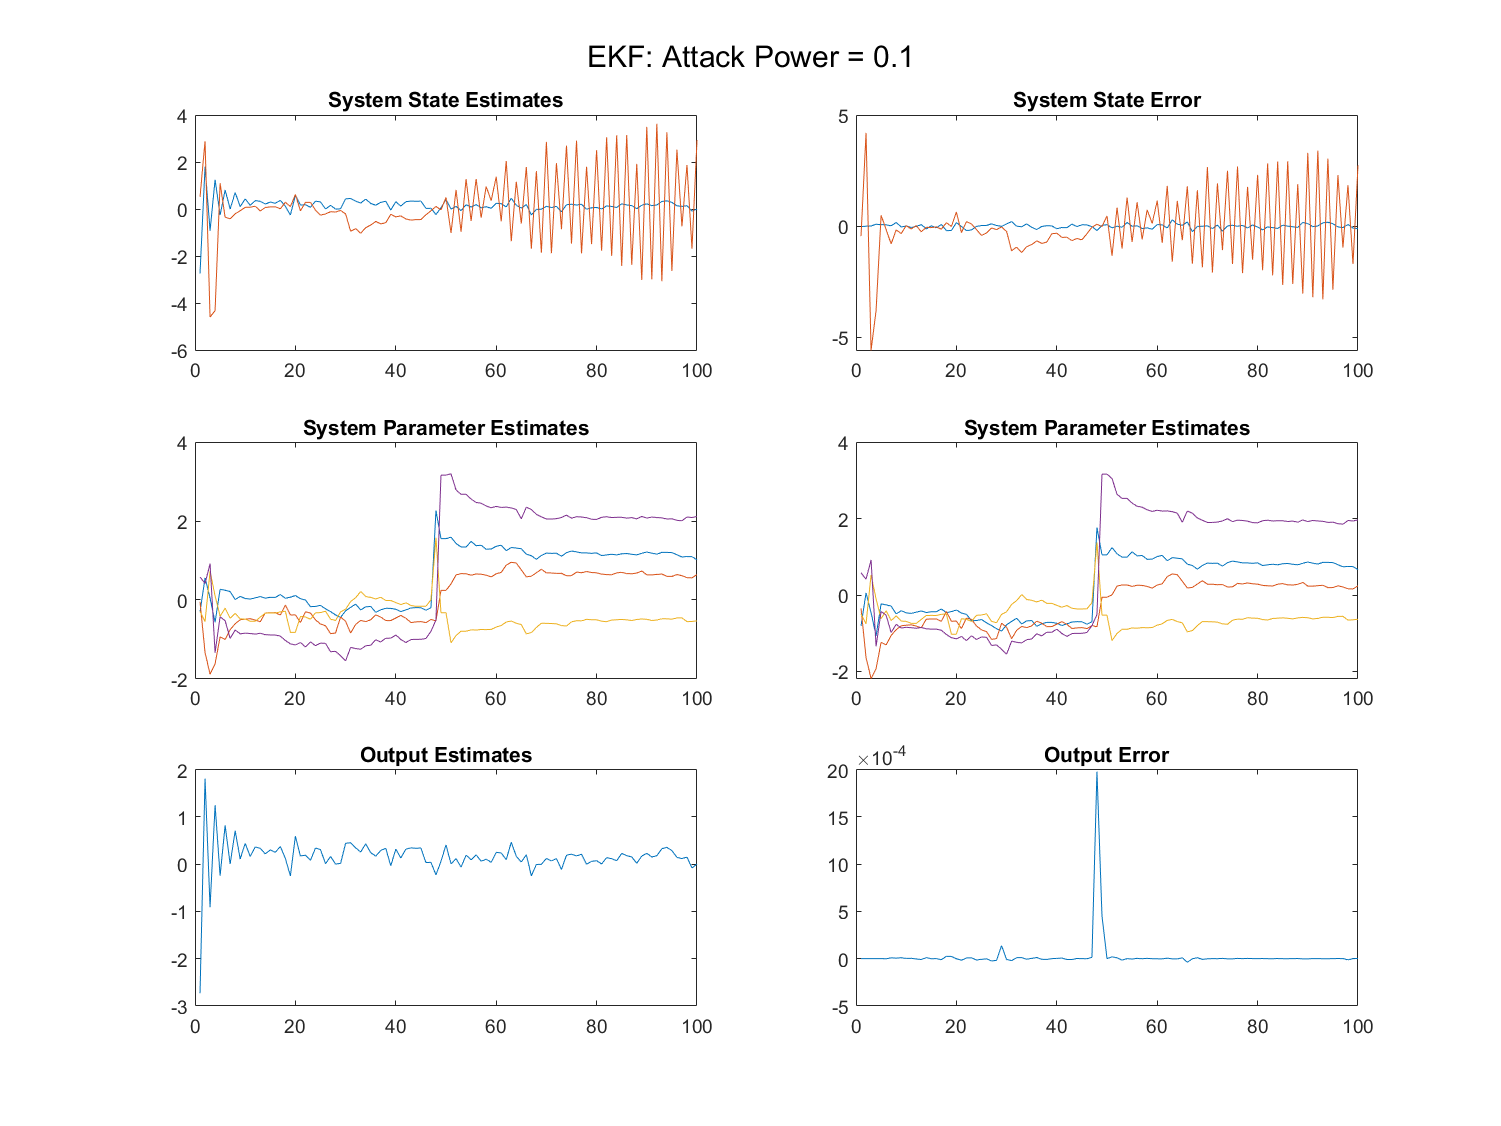
\includegraphics[width=\linewidth]{../../fig/EKF_attack_0_1}
	\caption{EKF with $v_0 = 0.1$ Simulated Results}
	\label{fig:ekfattack01}
\end{figure}

\begin{figure}
	\centering
	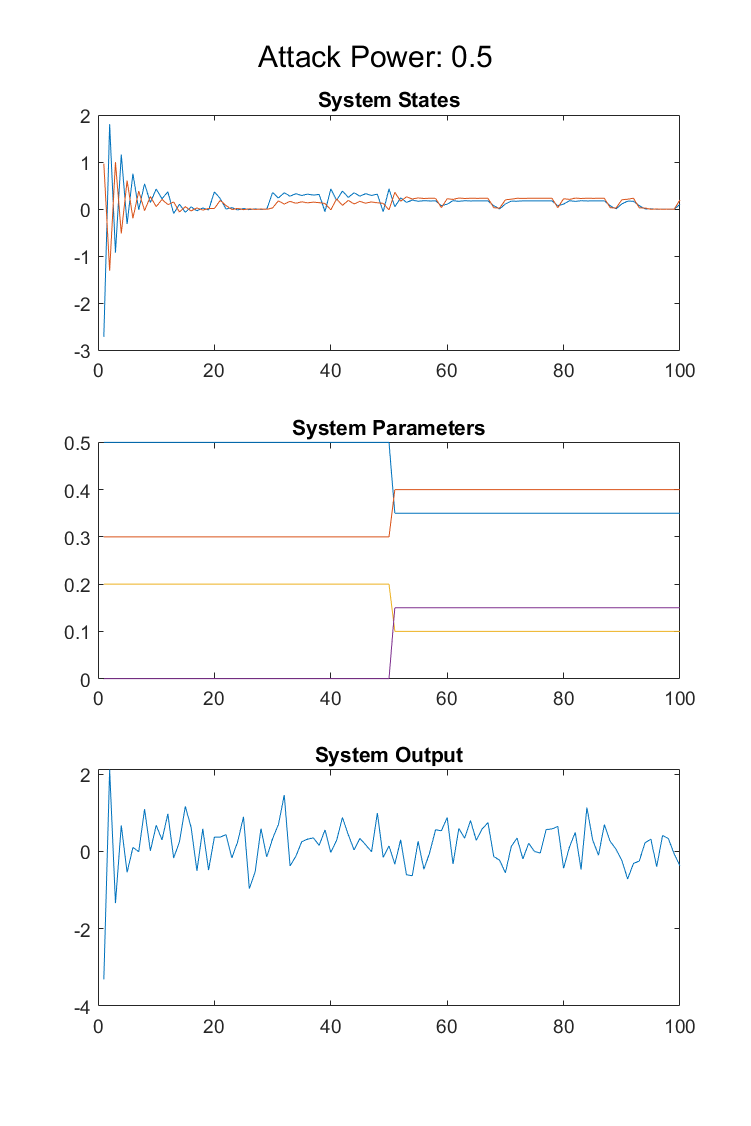
\includegraphics[width=0.7\linewidth]{../../fig/SystemResponse_attack_0_5}
	\caption{$v_0 = 0.5$ System Results}
	\label{fig:systemresponseattack05}
\end{figure}

\begin{figure}
	\centering
	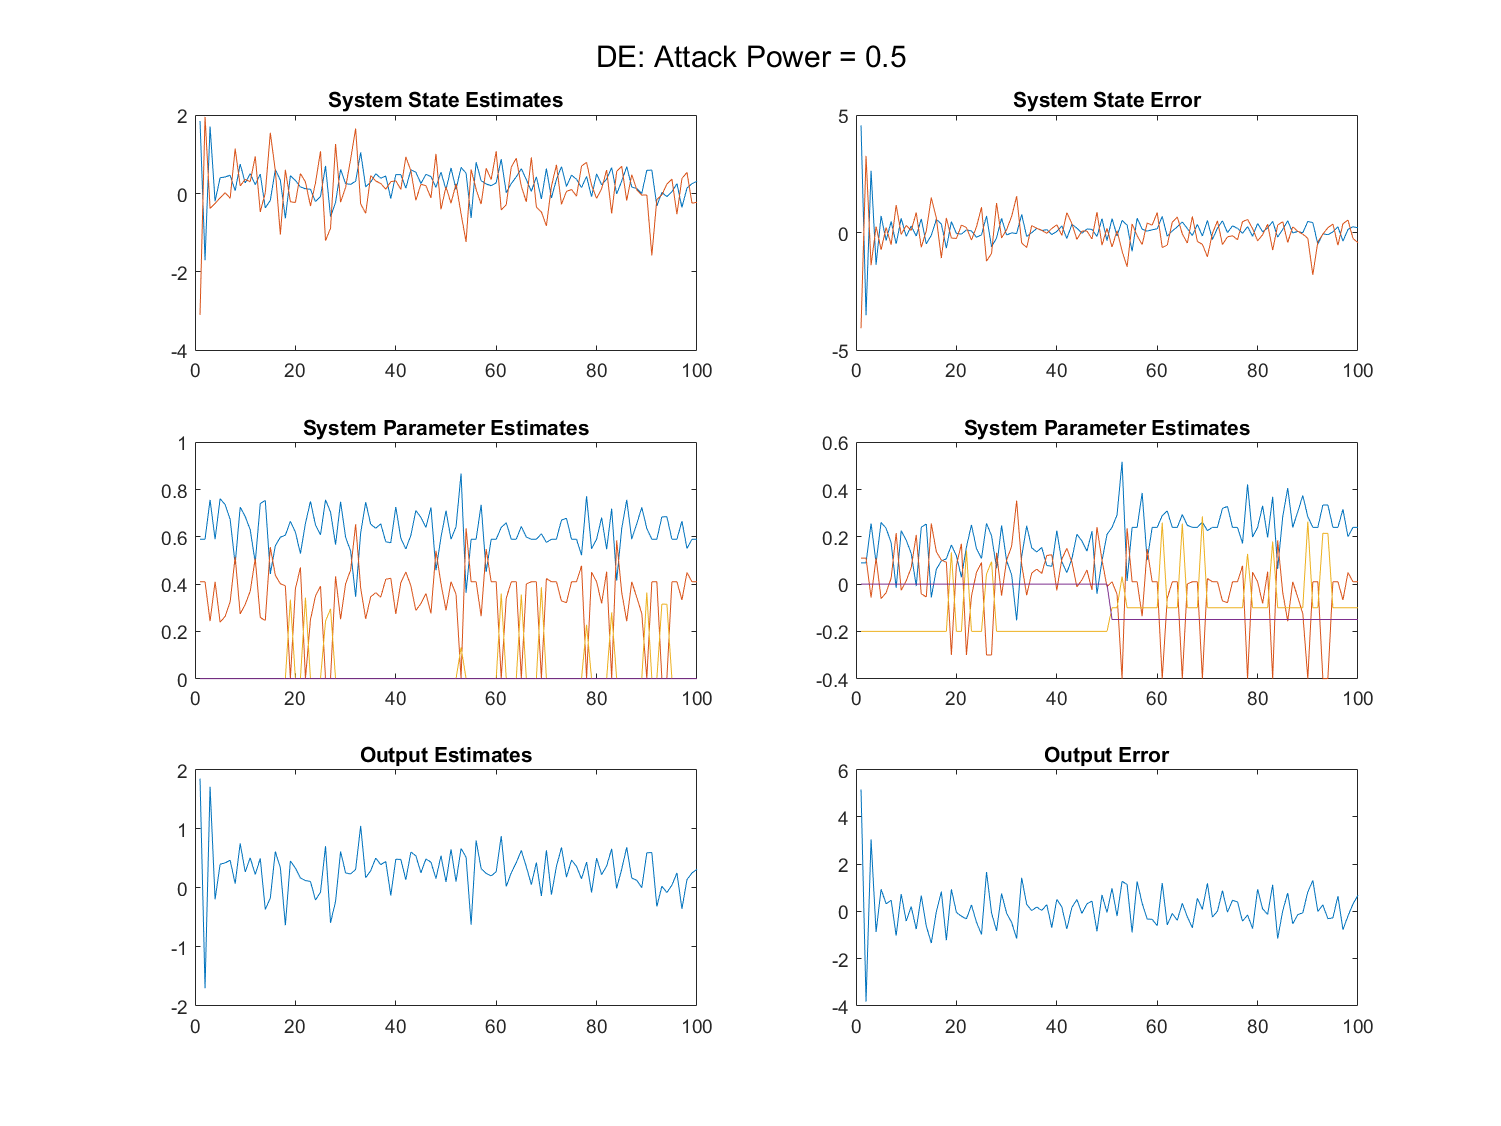
\includegraphics[width=\linewidth]{../../fig/DE_attack_0_5}
	\caption{DE with $v_0 = 0.5$ Simulated Results}
	\label{fig:deattack05}
\end{figure}

\begin{figure}
	\centering
	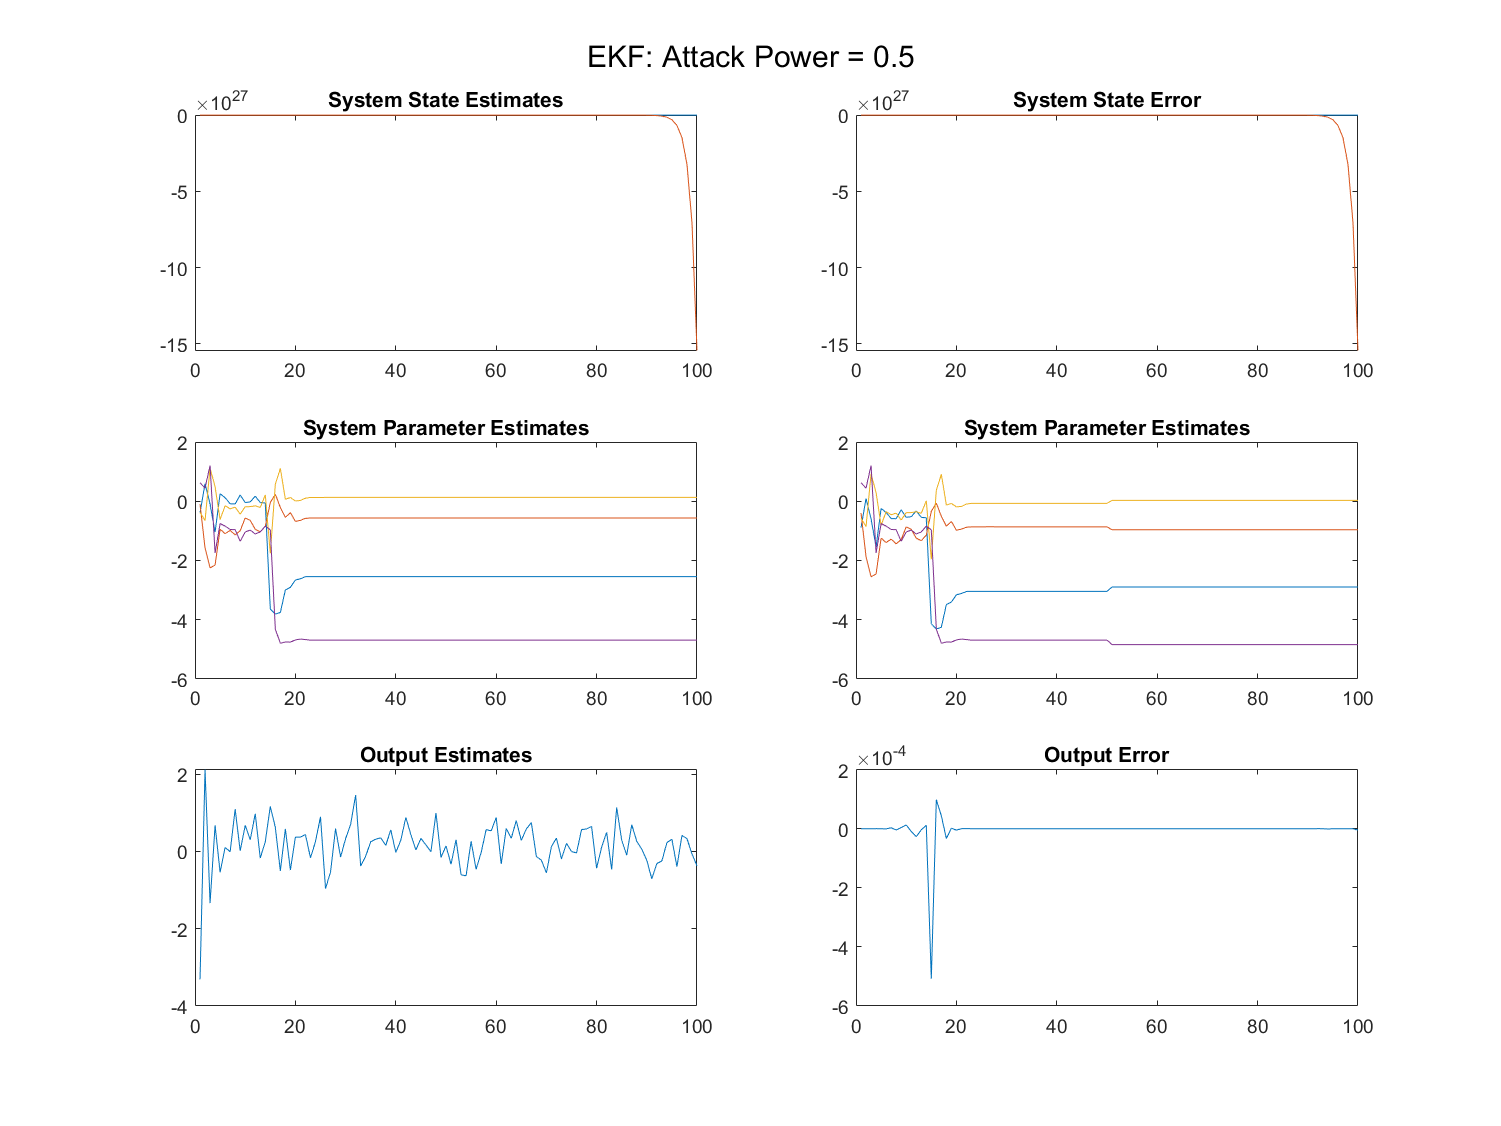
\includegraphics[width=\linewidth]{../../fig/EKF_attack_0_5}
	\caption{EKF with $v_0 = 0.5$ Simulated Results}
	\label{fig:ekfattack05}
\end{figure}



\end{document}
